\chapter{Architecture Frameworks, Descriptions and Languages}

This chapter briefly introduces concepts covered by ISO/IEC42010. It defines the terms used in the development of the architecture description artefact as well as discusses the architecture modeling language and frameworks used.


\section{Architecture \& Architecture Description}


ISO42010 and its predecessor IEEE1471 attempted to establish a coherent practice for developing architecture descriptions, frameworks and architecture description languages \cite{InternationalOrganizationOfStandardization2011}. This in turn required the formalization and standardization of key architecting terms (see table ISO Definitions \ref{table:iso_def} page~\pageref{table:iso_def}). One of the important distinctions made by these standards was that between architecture and architecture description (AD). In software, architecture refers to the fundamental concepts or properties of a system, in its environment and embodied in its elements, relationships and principles of its design and evolution \cite{InternationalOrganizationOfStandardization2011}. In order to explain this architecture and its components, architects produce a product of work that helps express the architecture as a whole namely an AD. ADs are powerful tools in expressing the core essence of a software system in relation to its key properties, behaviour, composition and evolution \cite{InternationalOrganizationOfStandardization2011}. 

Understanding this essence is also critical in helping us to bring into effect, manage and improve the system in regards to its non-functional requirements. These AD also help address known concerns for known stakeholders for a system of interest \cite{Emery2009}. It is therefore an important part of any software or systems life-cycle to produce some form of architectural description in order to communicate different concerns to the different stakeholders from their respective views throughout. The concerns of the different stakeholders are exemplified through the use of architectural views where each view covers a set of identified concerns and captured via the use of conceptual or meta-models \cite{42010faq}.


\section{Architecture Description Languages (ADLs)}

An ADL is a set of model, notations and specifications used that are applied in order to describe software architecture and its business domain for this paper a few ADLs have been considered including as the Stanford's Rapide Project \cite{Luckham1996}, WRIGHT ADL \cite{Allen1997} and ACME \cite{bjorn}. Although ADLs are popular amongst scholars and researchers their popularity amongst architects have been questionable outside specialized domains \cite{Woods2005}. In contrast, Unified Modeling Language or Unified Modeling Language (UML) has seen widespread adoption by system architects. Although it is not technically considered an ADL, UML provides a set of notations that suffice for creating of general architecture description models \cite{Woods2005}.

\section{UML}

UML was adopted as standard by the Object Management Group (OMG) in 1997. It is the result of a variety of Object-Oriented Analysis and Design methods that were introduced during the 80's and 90's \cite{Fowler2004}. Developed by a team of architects commonly referred to as the "three amigos", UML is a direct result of the work done by Grady Booch, Ivar Jacobson and James Rumbaugh at the Rational software company. After adoption as standard by OMG, UML has received widespread adoption and usage in software and enterprise systems architecture communities. UML2 includes 13 basic diagrams which are generally subdivided into two broad categories for modeling. Firstly, structural diagrams indicate static architectural constructs such as classes, objects and components as well as the relationship between these. Secondly, behavioural diagrams are used to model the functional or dynamic constructs of architecture. This thesis uses UML as its ADLs.


\section{Architectural Framework}

ISO/IEC/IEEE 42010:2011 (ISO-42010) defines an architecture framework as "a framework establishing a common practice for creating, interpreting, analyzing and using ADs within a particular domain of application or stakeholder community".

\begin{figure}
\centering
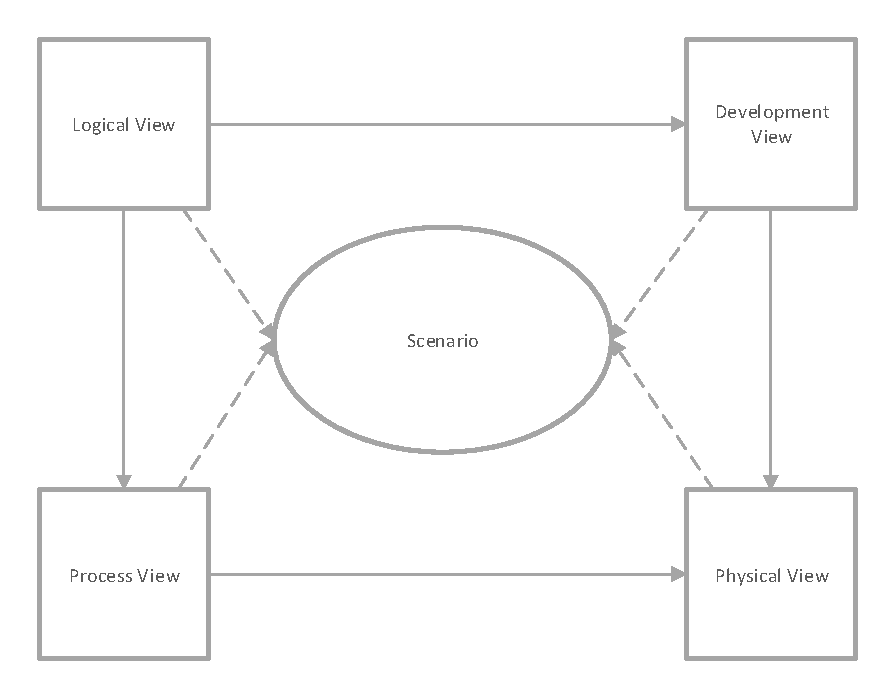
\includegraphics[width=\textwidth]{4plus1frameworksmall}
\caption{4 + 1 Framework}
\label{fig:4plus1frameworksmall}
\end{figure}

The 4+1 Architectural View Model as designed by Kruchten \cite{Kruchten} identified five high level views for use during the creation of an AD (see figure \ref{fig:4plus1frameworksmall}). These views correspond to ISO-42010's view points as they refer to different stakeholder's views and help address these stakeholders' specific considerations. It is important to note that although \cite{Kruchten} uses the term view in his work, ISO-42010 defines the view as the physical work product of an architectural view. A simple breakdown of the 4+1 viewpoints and their mappings to supportive UML diagrams can be seen in Appendix \ref{table:viewpoints} as a composition of \cite{Wiki4plus1}, \cite{Muchandi2007} and \cite{Kruchten}:


This thesis uses the 4+1 framework in order to define the common principles and practices for describing the architecture. This framework is combined with UML in order to provide specific viewpoints from which views are constructed via diagrams of various model types.

\section{Conclusion}

This chapter provided information on the practices of systems and software engineering in creation of an AD according to ISO-42010. It also discusses UML as ADL and Kruchten's 4+1 view model as architectural framework as used by this thesis.


